\documentclass[11pt]{article}
\usepackage[notes]{la}
\lamodule{4}{2}{Null, Column and Row Spaces; Linear Maps}
\laxdoc{1.2}
\laxdoc{1.4}
\laxdoc{1.5}
\laxdoc{1.8}
\laxdoc{1.9}
\laxdoc{2.1}
\laxdoc{2.3}
\laxdoc{4.1}

\begin{document}

\section{Null Spaces, Column Spaces, Row Spaces, and Linear Transformations}

\begin{guide}
Every matrix carries two subspaces of its own. For an $m\times n$ matrix $A$ you have asked two questions since Chapter 1. Which vectors $\bv{b}$ in $\R^m$ make $A\bv{x}=\bv{b}$ solvable? And when a solution exists, how much freedom is there among the solutions? The first question is answered by the \emph{column space} of $A$, the second by its \emph{null space}. Section 4.1 supplied the language of subspaces; this section applies it to matrices. Then the same two ideas are carried over to maps between polynomials, matrices and functions. In Section 1.8 a ``linear transformation'' was a map $\R^n\to\R^m$. Can the same two rules define linearity when the ``vectors'' are polynomials or functions, and what plays the role of the null space and the column space there?
\end{guide}

\textbf{By the end of this section you should be able to:}
\begin{itemize}
  \item define $\Nul A$, $\Col A$ and $\Row A$, say which $\R^k$ each lives in, and prove that each is a subspace;
  \item find a spanning set for $\Nul A$ from the free variables, and test whether a given vector lies in $\Nul A$ by multiplying;
  \item decide whether $\bv{b}$ lies in $\Col A$ by row reducing $[A\ \bv{b}]$, including when $\bv{b}$ has a parameter, and say when $\Col A=\R^m$;
  \item read $\Row A$ off an echelon form, and explain why row operations leave $\Nul A$ and $\Row A$ unchanged but \emph{do} change $\Col A$;
  \item compare $\Nul A$ and $\Col A$ for one matrix, and decide whether a set is a subspace by writing it as $\Nul A$ or $\Col A$;
  \item define a linear transformation between vector spaces, find its kernel and range, and use the criterion ``one-to-one if and only if the kernel is $\{\bv{0}\}$''.
\end{itemize}

% ---------------------------------------------------------------------
\subsection*{A first look}

\begin{exmp}{Two lines from one matrix}{firstlook}
Let $A=\begin{bmatrix}1&2\\2&4\end{bmatrix}$. For every $\bv{x}=(x_1,x_2)$ the product is
\[
A\bv{x}=x_1\begin{bmatrix}1\\2\end{bmatrix}+x_2\begin{bmatrix}2\\4\end{bmatrix}=(x_1+2x_2)\begin{bmatrix}1\\2\end{bmatrix},
\]
so every value of $A\bv{x}$ is a multiple of $(1,2)$: the equation $A\bv{x}=\bv{b}$ is solvable exactly when $\bv{b}$ lies on the line $\Span\{(1,2)\}$ (the line $y=2x$). On the other hand $A\bv{x}=\bv{0}$ means $x_1+2x_2=0$, so $\bv{x}=x_2(-2,1)$: the solutions are the line $\Span\{(-2,1)\}$. Two lines through the origin, both subspaces of $\R^2$, but with different jobs. The first line lives in the space of \emph{outputs} (where the $\bv{b}$ live) and the second in the space of \emph{inputs} (where the $\bv{x}$ live). It is only an accident of this matrix being $2\times2$ that both inputs and outputs are vectors of $\R^2$.
\end{exmp}

% ---------------------------------------------------------------------
\subsection*{The null space}

\begin{defn}{Null space}{nul}
The \emph{null space} of an $m\times n$ matrix $A$, written $\Nul A$, is the set of all solutions of the homogeneous equation $A\bv{x}=\bv{0}$:
\[
\Nul A=\{\bv{x}\in\R^n:\ A\bv{x}=\bv{0}\}.
\]
\end{defn}

The vectors $\bv{x}$ must have $n$ entries for $A\bv{x}$ to be defined, so $\Nul A$ is a subset of $\R^n$, where $n$ is the number of \emph{columns}. In Section 1.5 you studied this set under the name ``solution set of $A\bv{x}=\bv{0}$''. What is new is the question we can now ask of it.

\begin{thm}{The null space is a subspace}{nulsub}
For every $m\times n$ matrix $A$, the set $\Nul A$ is a subspace of $\R^n$.
\end{thm}

\begin{proof}
\textbf{First proof: linearity of $A\bv{x}$.} The zero vector is in $\Nul A$, because $A\bv{0}=\bv{0}$ (every weight in the combination of the columns is $0$, Definition~\ref{1.4-def:matvec}). Let $\bv{u},\bv{v}$ be in $\Nul A$ and let $c$ be a scalar. By Theorem~\ref{1.4-thm:linear},
\[
A(\bv{u}+\bv{v})=A\bv{u}+A\bv{v}=\bv{0}+\bv{0}=\bv{0},\qquad A(c\bv{u})=c(A\bv{u})=c\bv{0}=\bv{0},
\]
where $c\bv{0}=\bv{0}$ is Theorem~\ref{4.1-thm:conseq}(d). So $\Nul A$ satisfies (a), (b), (c) of Definition~\ref{4.1-def:subspace}.

\textbf{Second proof: the Subspace Test, one equation at a time.} Write the $m$ equations of $A\bv{x}=\bv{0}$ as $a_{i1}x_1+\cdots+a_{in}x_n=0$ for $i=1,\dots,m$. A vector is in $\Nul A$ exactly when its entries satisfy all $m$ equations. (a)~The zero vector satisfies each equation, since every term is $0$. (b)~If $\bv{u}$ and $\bv{v}$ satisfy equation $i$, then
\[
a_{i1}(u_1+v_1)+\cdots+a_{in}(u_n+v_n)=(a_{i1}u_1+\cdots+a_{in}u_n)+(a_{i1}v_1+\cdots+a_{in}v_n)=0+0=0,
\]
for every $i$, so $\bv{u}+\bv{v}$ is in $\Nul A$. (c)~Likewise $a_{i1}(cu_1)+\cdots+a_{in}(cu_n)=c\,(a_{i1}u_1+\cdots+a_{in}u_n)=0$. This is the computation of Example~\ref{4.1-ex:plane}, done for $m$ equations at once. By the Subspace Test (Theorem~\ref{4.1-thm:subtest}), $\Nul A$ is a subspace of $\R^n$.
\end{proof}

\begin{remark}[Implicit versus explicit]
The null space is described \emph{implicitly}: it is the set of vectors that satisfy a condition, $A\bv{x}=\bv{0}$. An implicit description tells you how to \emph{test} a vector (multiply by $A$) but not how to \emph{produce} one. An \emph{explicit} description, such as ``all combinations $c_1\bv{v}_1+\cdots+c_k\bv{v}_k$'', produces every vector at once, as a span does. The parametric vector form of Section 1.5 converts the first kind of description into the second: each free variable becomes a weight. Theorem~\ref{thm:nulsub} says the result is always a span, so the conversion is always possible.
\end{remark}

\begin{proc}{A spanning set for $\Nul A$}{nulspan}
\begin{enumerate}
  \item Row reduce $[A\ \bv{0}]$ (equivalently $A$) to reduced echelon form.
  \item Identify the free variables and write each basic variable in terms of them.
  \item Write the general solution in parametric vector form $\bv{x}=x_{j_1}\bv{v}_1+\cdots+x_{j_k}\bv{v}_k$ (Procedure~\ref{1.5-proc:pvf}; the constant vector is $\bv{0}$ because the right-hand side is $\bv{0}$).
  \item Then $\Nul A=\Span\{\bv{v}_1,\dots,\bv{v}_k\}$: one vector for each free variable. If there is no free variable, $\Nul A=\{\bv{0}\}$.
  \item Check each $\bv{v}_i$ by computing $A\bv{v}_i$.
\end{enumerate}
\end{proc}

\begin{exmp}{A $2\times4$ matrix with two free variables}{nul24}
Find a spanning set for $\Nul A$, where $A=\begin{bmatrix}1&-2&1&0\\2&-4&3&1\end{bmatrix}$.

\textbf{Solution.} Row reduce $[A\ \bv{0}]$:
\begin{align*}
\begin{amat}{cccc|c}1&-2&1&0&0\\2&-4&3&1&0\end{amat}
&\rops{R_2-2R_1}
\begin{amat}{cccc|c}1&-2&1&0&0\\0&0&1&1&0\end{amat}
\rops{R_1-R_2}
\begin{amat}{cccc|c}1&-2&0&-1&0\\0&0&1&1&0\end{amat}.
\end{align*}
The pivot columns are $1$ and $3$, so $x_2,x_4$ are free, with $x_1=2x_2+x_4$ and $x_3=-x_4$. Then
\[
\bv{x}=\begin{bmatrix}2x_2+x_4\\x_2\\-x_4\\x_4\end{bmatrix}=x_2\begin{bmatrix}2\\1\\0\\0\end{bmatrix}+x_4\begin{bmatrix}1\\0\\-1\\1\end{bmatrix},
\]
so $\Nul A=\Span\{(2,1,0,0),(1,0,-1,1)\}$, a subspace of $\R^4$. Check: $A(2,1,0,0)=(2-2,\ 4-4)=(0,0)$ and $A(1,0,-1,1)=(1-1,\ 2-3+1)=(0,0)$. \ $\checkmark$
\end{exmp}

\begin{exmp}{A $3\times5$ matrix with three free variables}{nul35}
Let $A=\begin{bmatrix}1&1&0&2&-1\\0&0&1&-1&3\\1&1&1&1&2\end{bmatrix}$. Find a spanning set for $\Nul A$ and say in which $\R^k$ it lives.

\textbf{Solution.} Because $A$ has $5$ columns, $\Nul A$ is a subspace of $\R^5$. Row reduce:
\begin{align*}
\begin{amat}{ccccc|c}1&1&0&2&-1&0\\0&0&1&-1&3&0\\1&1&1&1&2&0\end{amat}
&\rops{R_3-R_1}
\begin{amat}{ccccc|c}1&1&0&2&-1&0\\0&0&1&-1&3&0\\0&0&1&-1&3&0\end{amat}\\[4pt]
&\rops{R_3-R_2}
\begin{amat}{ccccc|c}1&1&0&2&-1&0\\0&0&1&-1&3&0\\0&0&0&0&0&0\end{amat}.
\end{align*}
This is already reduced. The pivot columns are $1$ and $3$; the free variables are $x_2,x_4,x_5$, with $x_1=-x_2-2x_4+x_5$ and $x_3=x_4-3x_5$. So
\[
\bv{x}=x_2\begin{bmatrix}-1\\1\\0\\0\\0\end{bmatrix}+x_4\begin{bmatrix}-2\\0\\1\\1\\0\end{bmatrix}+x_5\begin{bmatrix}1\\0\\-3\\0\\1\end{bmatrix}.
\]
Hence $\Nul A=\Span\{(-1,1,0,0,0),\ (-2,0,1,1,0),\ (1,0,-3,0,1)\}$. Check the middle vector: $A(-2,0,1,1,0)=(-2+0+0+2+0,\ 0+0+1-1+0,\ -2+0+1+1+0)=(0,0,0)$. \ $\checkmark$ Each free variable appears as a $1$ in its own position of exactly one spanning vector, and as a $0$ in the others; this is why no spanning vector is a combination of the other two.
\end{exmp}

\begin{exmp}{When the null space is the zero subspace}{nulzero}
Let $A=\begin{bmatrix}1&2\\0&1\\1&3\end{bmatrix}$. Find $\Nul A$.

\textbf{Solution.} Since $A$ has $2$ columns, $\Nul A$ lives in $\R^2$. Row reduce:
\begin{align*}
\begin{amat}{cc|c}1&2&0\\0&1&0\\1&3&0\end{amat}
&\rops{R_3-R_1}
\begin{amat}{cc|c}1&2&0\\0&1&0\\0&1&0\end{amat}
\rops{R_3-R_2}
\begin{amat}{cc|c}1&2&0\\0&1&0\\0&0&0\end{amat}.
\end{align*}
Both columns are pivot columns, so there is no free variable, $x_2=0$ and $x_1=0$: $\Nul A=\{\bv{0}\}$. By Theorem~\ref{1.5-thm:nontriv} this is exactly the situation in which $A\bv{x}=\bv{0}$ has only the trivial solution, and by Theorem~\ref{1.9-thm:ontoone}(a) it says that $\bv{x}\mapsto A\bv{x}$ is one-to-one. The zero subspace is a legitimate subspace (Example~\ref{4.1-ex:chain}); it is the answer, not a sign that something went wrong.
\end{exmp}

\begin{exmp}{A single equation: a plane}{nulplane}
Let $A=\begin{bmatrix}1&-2&1\end{bmatrix}$, a $1\times3$ matrix. Then $A\bv{x}=\bv{0}$ is the single equation $x_1-2x_2+x_3=0$, so $\Nul A=\{(a,b,c):\ a-2b+c=0\}$, which is the plane $H$ of Example~\ref{4.1-ex:plane}. The matrix is already in reduced echelon form with one pivot column, so $x_2,x_3$ are free and $x_1=2x_2-x_3$:
\[
\bv{x}=x_2\begin{bmatrix}2\\1\\0\end{bmatrix}+x_3\begin{bmatrix}-1\\0\\1\end{bmatrix}.
\]
This is the spanning set found in Example~\ref{4.1-ex:restriction}(a), by the same computation. Conversely, \emph{every} plane through the origin in $\R^3$ that is given by one equation is the null space of a $1\times3$ matrix, and a line through the origin given by two equations is the null space of a $2\times3$ matrix.
\end{exmp}

\begin{exmp}{Testing a vector by multiplying}{nultest}
Let $A=\begin{bmatrix}1&-1&2&0\\0&1&-1&3\\1&0&1&3\end{bmatrix}$. Which of $\bv{u}=(-4,-2,1,1)$ and $\bv{v}=(1,1,1,1)$ lie in $\Nul A$?

\textbf{Solution.} A vector is in $\Nul A$ if and only if $A\bv{x}=\bv{0}$, so multiply:
\[
A\bv{u}=\begin{bmatrix}1&-1&2&0\\0&1&-1&3\\1&0&1&3\end{bmatrix}\begin{bmatrix}-4\\-2\\1\\1\end{bmatrix}=\begin{bmatrix}-4+2+2+0\\0-2-1+3\\-4+0+1+3\end{bmatrix}=\begin{bmatrix}0\\0\\0\end{bmatrix},
\]
\[
A\bv{v}=\begin{bmatrix}1&-1&2&0\\0&1&-1&3\\1&0&1&3\end{bmatrix}\begin{bmatrix}1\\1\\1\\1\end{bmatrix}=\begin{bmatrix}1-1+2+0\\0+1-1+3\\1+0+1+3\end{bmatrix}=\begin{bmatrix}2\\3\\5\end{bmatrix}.
\]
So $\bv{u}$ is in $\Nul A$ and $\bv{v}$ is not. No row reduction is needed for a membership test in $\Nul A$; row reduction is needed to \emph{describe} all of $\Nul A$. (Row reducing $A$ gives the free variables $x_3,x_4$ and the spanning set $\{(-1,1,1,0),(-3,-3,0,1)\}$, and indeed $\bv{u}=(-1,1,1,0)+(-3,-3,0,1)$.)
\end{exmp}

\begin{kc}{Which $\R^k$?}{shapes}
For each matrix shape, say in which $\R^k$ the null space lives and in which $\R^k$ the column space lives: (a)~$3\times5$; (b)~$4\times2$; (c)~$6\times6$; (d)~$1\times7$.
\end{kc}

\begin{kc}{Read off a spanning set}{readnul}
Each matrix is the reduced echelon form of $A$. Write $\Nul A$ as a span (or say it is $\{\bv{0}\}$), and say in which $\R^k$ it lives. (a)~$\begin{bmatrix}1&0&3\\0&1&-2\end{bmatrix}$. (b)~$\begin{bmatrix}1&2&0&-1\\0&0&1&4\end{bmatrix}$. (c)~$\begin{bmatrix}1&0\\0&1\\0&0\end{bmatrix}$.
\end{kc}

\begin{center}
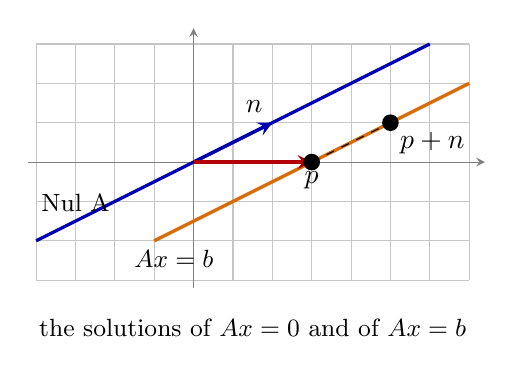
\begin{tikzpicture}[x=0.5cm,y=0.5cm,>=stealth]
  \draw[gray!45] (-4,-3) grid[step=1] (7,3);
  \draw[->,gray] (-4.2,0)--(7.4,0);
  \draw[->,gray] (0,-3.2)--(0,3.4);
  \draw[very thick,blue!70!black] (-4,-2)--(6,3);
  \draw[very thick,orange!85!black] (-1,-2)--(7,2);
  \draw[->,very thick,blue!70!black] (0,0)--(2,1);
  \node[above left] at (2,1) {$n$};
  \draw[->,very thick,red!70!black] (0,0)--(3,0);
  \fill (3,0) circle (3pt);
  \node[below] at (3,0) {$p$};
  \draw[dashed] (3,0)--(5,1);
  \fill (5,1) circle (3pt);
  \node[below right] at (5,1) {$p+n$};
  \node[above] at (-3,-1.5) {\small Nul A};
  \node[below] at (-0.5,-2) {\small $Ax=b$};
  \node at (1.5,-4.2) {\small the solutions of $Ax=0$ and of $Ax=b$};
\end{tikzpicture}
\end{center}

\textbf{Figure 1.} Let $A=\begin{bmatrix}1&-2\end{bmatrix}$ and $b=3$, so $A\bv{x}=b$ is the equation $x_1-2x_2=3$. The blue line is $\Nul A$, the solutions of $x_1-2x_2=0$; it passes through the origin and contains $\bv{n}=(2,1)$. The orange line is the solution set of $A\bv{x}=3$; it contains $\bv{p}=(3,0)$ and is the blue line moved by $\bv{p}$: its points are $\bv{p}+\bv{n}$ with $\bv{n}$ in $\Nul A$ (Theorem~\ref{1.5-thm:translate}), such as $\bv{p}+\bv{n}=(5,1)$. The orange line misses the origin, so it is not a subspace.

\begin{think}{A subspace, but the solutions of $A\bv{x}=\bv{b}$ are not}{shifted}
The set $\Nul A$ of solutions of $A\bv{x}=\bv{0}$ is a subspace. Take $A=\begin{bmatrix}1&-2&1\end{bmatrix}$ and $\bv{b}=(2)$, so that $A\bv{x}=\bv{b}$ is the equation $x_1-2x_2+x_3=2$. Is its solution set a subspace of $\R^3$? Which property fails, and how does that failure relate to the shifted plane of Example~\ref{4.1-ex:shifted} (the right half of Figure 1 in Section 4.1) and to Theorem~\ref{1.5-thm:translate}? (Figure 1 below, in this section, shows the same phenomenon in the plane.)
\end{think}

% ---------------------------------------------------------------------
\subsection*{The column space}

\begin{defn}{Column space}{col}
The \emph{column space} of an $m\times n$ matrix $A=\begin{bmatrix}\bv{a}_1&\cdots&\bv{a}_n\end{bmatrix}$, written $\Col A$, is the set of all linear combinations of the columns of $A$:
\[
\Col A=\Span\{\bv{a}_1,\dots,\bv{a}_n\}.
\]
\end{defn}

Each column of $A$ has $m$ entries, so $\Col A$ is a subset of $\R^m$, where $m$ is the number of \emph{rows}. The column space is described explicitly (as a span), and the work is in the membership test.

\begin{thm}{Three descriptions of the column space}{colsub}
Let $A$ be an $m\times n$ matrix.
\begin{enumerate}[label=(\alph*),itemsep=1pt]
  \item $\Col A$ is a subspace of $\R^m$.
  \item $\Col A=\{A\bv{x}:\ \bv{x}\in\R^n\}$, the set of all values of $A\bv{x}$.
  \item $\Col A=\{\bv{b}\in\R^m:\ A\bv{x}=\bv{b}\text{ has a solution}\}$.
\end{enumerate}
\end{thm}

\begin{proof}
(a)~A span is a subspace (Theorem~\ref{4.1-thm:spansub}), here of $\R^m$. (b)~By Definition~\ref{1.4-def:matvec}, $A\bv{x}=x_1\bv{a}_1+\cdots+x_n\bv{a}_n$, and as $\bv{x}$ runs over $\R^n$ the weights $x_1,\dots,x_n$ run over all lists of $n$ real numbers, so the values $A\bv{x}$ are exactly the linear combinations of the columns. (c)~A vector $\bv{b}$ is of the form $A\bv{x}$ if and only if the equation $A\bv{x}=\bv{b}$ has a solution; this is part (b) restated (compare Theorem~\ref{1.4-thm:three}).
\end{proof}

Part (c) is the answer to the first question of the guide: \emph{$\Col A$ is the set of right-hand sides $\bv{b}$ for which $A\bv{x}=\bv{b}$ is consistent.} To decide whether a given $\bv{b}$ is in $\Col A$ we therefore row reduce $[A\ \bv{b}]$ and look for a pivot in the last column (Theorem~\ref{1.2-thm:existuniq}).

\begin{exmp}{Is $\bv{b}$ in $\Col A$?}{colmember}
Let $A=\begin{bmatrix}1&0&1\\2&1&3\\-1&1&0\end{bmatrix}$. Which of $\bv{b}_1=(2,7,1)$ and $\bv{b}_2=(1,1,1)$ lie in $\Col A$?

\textbf{Solution.} Because $A$ has $3$ rows, $\Col A$ is a subspace of $\R^3$, and so are both $\bv{b}_i$; the question is meaningful. For $\bv{b}_1$:
\begin{align*}
\begin{amat}{ccc|c}1&0&1&2\\2&1&3&7\\-1&1&0&1\end{amat}
&\rops{R_2-2R_1,\ R_3+R_1}
\begin{amat}{ccc|c}1&0&1&2\\0&1&1&3\\0&1&1&3\end{amat}
\rops{R_3-R_2}
\begin{amat}{ccc|c}1&0&1&2\\0&1&1&3\\0&0&0&0\end{amat}.
\end{align*}
The last column is not a pivot column, so $A\bv{x}=\bv{b}_1$ is consistent and $\bv{b}_1$ is in $\Col A$. The third column is free, so the weights are not unique: $x_1=2-x_3$, $x_2=3-x_3$. With $x_3=0$ we get $\bv{b}_1=2\bv{a}_1+3\bv{a}_2=2(1,2,-1)+3(0,1,1)=(2,7,1)$. \ $\checkmark$ For $\bv{b}_2$:
\begin{align*}
\begin{amat}{ccc|c}1&0&1&1\\2&1&3&1\\-1&1&0&1\end{amat}
&\rops{R_2-2R_1,\ R_3+R_1}
\begin{amat}{ccc|c}1&0&1&1\\0&1&1&-1\\0&1&1&2\end{amat}
\rops{R_3-R_2}
\begin{amat}{ccc|c}1&0&1&1\\0&1&1&-1\\0&0&0&3\end{amat}.
\end{align*}
The last row says $0=3$, so $A\bv{x}=\bv{b}_2$ is inconsistent and $\bv{b}_2$ is \emph{not} in $\Col A$.
\end{exmp}

\begin{exmp}{A parameter in $\bv{b}$}{colparam}
Let $A=\begin{bmatrix}1&0&1\\0&1&1\\1&1&2\end{bmatrix}$ and $\bv{b}=(2,-1,k)$. For which $k$ is $\bv{b}$ in $\Col A$?

\textbf{Solution.}
\begin{align*}
\begin{amat}{ccc|c}1&0&1&2\\0&1&1&-1\\1&1&2&k\end{amat}
&\rops{R_3-R_1}
\begin{amat}{ccc|c}1&0&1&2\\0&1&1&-1\\0&1&1&k-2\end{amat}
\rops{R_3-R_2}
\begin{amat}{ccc|c}1&0&1&2\\0&1&1&-1\\0&0&0&k-1\end{amat}.
\end{align*}
The system is consistent exactly when $k-1=0$. So $\bv{b}\in\Col A$ if and only if $k=1$; then $x_1=2-x_3$, $x_2=-1-x_3$, and with $x_3=0$ we have $(2,-1,1)=2\bv{a}_1-\bv{a}_2=(2,0,2)-(0,1,1)$. \ $\checkmark$ Geometrically: the third column is the sum of the first two, so $\Col A=\Span\{\bv{a}_1,\bv{a}_2\}=\{(x,y,x+y)\}$ is a plane in $\R^3$, and the vector $(2,-1,k)$ is on the plane only when its third entry equals $2+(-1)=1$.
\end{exmp}

\begin{thm}{When is $\Col A=\R^m$?}{colall}
For an $m\times n$ matrix $A$ the following statements are equivalent.
\begin{enumerate}[label=(\alph*),itemsep=1pt]
  \item $\Col A=\R^m$.
  \item The equation $A\bv{x}=\bv{b}$ has a solution for every $\bv{b}$ in $\R^m$.
  \item $A$ has a pivot in every row.
\end{enumerate}
If $A$ is square ($m=n$), these statements are equivalent to $A$ being invertible: they are statements (g) and (h) of the Invertible Matrix Theorem (Theorem~\ref{2.3-thm:imt}).
\end{thm}

\begin{proof}
(a)$\iff$(b) is Theorem~\ref{thm:colsub}(c): $\Col A$ consists of the $\bv{b}$ for which $A\bv{x}=\bv{b}$ has a solution, so it is all of $\R^m$ exactly when every $\bv{b}$ has one. (b)$\iff$(c) is the equivalence of (a) and (d) in Theorem~\ref{1.4-thm:existence}. The last sentence is Theorem~\ref{2.3-thm:imt}, where (g) says that $A\bv{x}=\bv{b}$ has a solution for every $\bv{b}$ and (h) says that the columns of $A$ span $\R^n$.
\end{proof}

\begin{think}{When is the column space everything?}{colall}
(a)~A $3\times4$ matrix has a pivot in every row. What is $\Col A$? Does it depend on the entries of $A$? (b)~A $4\times3$ matrix: can $\Col A=\R^4$? (Count pivots.) (c)~If $A$ is $n\times n$ and $\Col A\neq\R^n$, what else do you know about $A$ from Theorem~\ref{2.3-thm:imt}?
\end{think}

\begin{exmp}{A column space equal to $\R^3$}{colsurj}
Let $A=\begin{bmatrix}1&2&0&1\\0&1&1&-1\\2&5&1&0\end{bmatrix}$. Show that $\Col A=\R^3$, and solve $A\bv{x}=(3,0,5)$.

\textbf{Solution.} Row reduce $A$ alone to see the pivot positions:
\begin{align*}
\begin{amat}{cccc}1&2&0&1\\0&1&1&-1\\2&5&1&0\end{amat}
&\rops{R_3-2R_1}
\begin{amat}{cccc}1&2&0&1\\0&1&1&-1\\0&1&1&-2\end{amat}
\rops{R_3-R_2}
\begin{amat}{cccc}1&2&0&1\\0&1&1&-1\\0&0&0&-1\end{amat}.
\end{align*}
The pivots are in columns $1$, $2$ and $4$, one in each of the three rows. By Theorem~\ref{thm:colall}, $\Col A=\R^3$: no right-hand side can produce a row $0=\text{nonzero}$. To see it concretely for $\bv{b}=(3,0,5)$:
\begin{align*}
\begin{amat}{cccc|c}1&2&0&1&3\\0&1&1&-1&0\\2&5&1&0&5\end{amat}
&\rops{R_3-2R_1}
\begin{amat}{cccc|c}1&2&0&1&3\\0&1&1&-1&0\\0&1&1&-2&-1\end{amat}
\rops{R_3-R_2}
\begin{amat}{cccc|c}1&2&0&1&3\\0&1&1&-1&0\\0&0&0&-1&-1\end{amat}.
\end{align*}
Back substitution gives $x_4=1$, $x_2=1-x_3$, $x_1=2x_3$. With $x_3=0$: $\bv{x}=(0,1,0,1)$, and $A\bv{x}=\bv{a}_2+\bv{a}_4=(2,1,5)+(1,-1,0)=(3,0,5)$. \ $\checkmark$ There are four columns for three rows, so there is a free variable too: many solutions, and a solution for every $\bv{b}$.
\end{exmp}

\begin{exmp}{A column space that is a plane}{colplane}
Let $B=\begin{bmatrix}1&0\\2&1\\-1&1\end{bmatrix}$. Describe $\Col B\subset\R^3$ by an equation.

\textbf{Solution.} $\Col B=\Span\{(1,2,-1),(0,1,1)\}$ is spanned by two vectors that are not multiples of each other, so it is a plane through the origin in $\R^3$. To find its equation, ask for which $\bv{b}=(b_1,b_2,b_3)$ the system $B\bv{x}=\bv{b}$ is consistent, keeping $b_1,b_2,b_3$ as symbols:
\begin{align*}
\begin{amat}{cc|c}1&0&b_1\\2&1&b_2\\-1&1&b_3\end{amat}
&\rops{R_2-2R_1,\ R_3+R_1}
\begin{amat}{cc|c}1&0&b_1\\0&1&b_2-2b_1\\0&1&b_3+b_1\end{amat}
\rops{R_3-R_2}
\begin{amat}{cc|c}1&0&b_1\\0&1&b_2-2b_1\\0&0&3b_1-b_2+b_3\end{amat}.
\end{align*}
The system is consistent if and only if $3b_1-b_2+b_3=0$, so $\Col B=\{(b_1,b_2,b_3):\ 3b_1-b_2+b_3=0\}$. Check: $\bv{b}=(1,3,0)=\bv{a}_1+\bv{a}_2$ satisfies $3-3+0=0$, while $\bv{c}=(0,0,4)$ gives $4\neq0$ and is not in $\Col B$. The matrix $A$ of Example~\ref{ex:colmember} has the same plane as its column space, because its third column is $\bv{a}_3=\bv{a}_1+\bv{a}_2$: the extra column adds nothing. The test of Example~\ref{ex:colmember} agrees: $(2,7,1)$ gives $6-7+1=0$, $(1,1,1)$ gives $3-1+1=3\neq0$.
\end{exmp}

\begin{center}
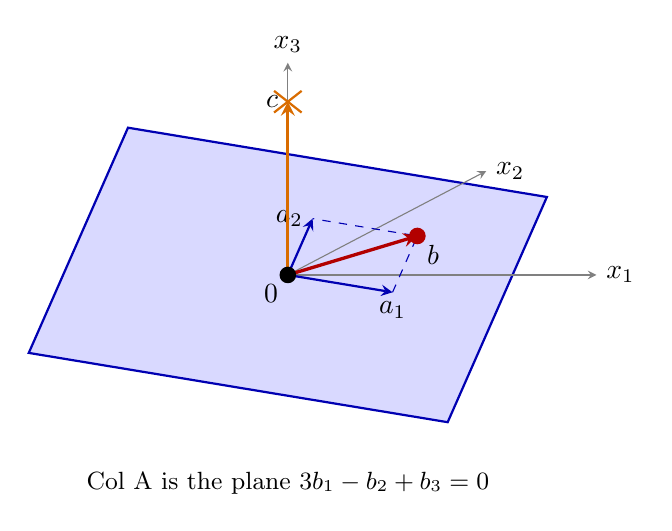
\begin{tikzpicture}[x=0.7cm,y=0.55cm,>=stealth]
  % oblique projection: the point (x1,x2,x3) is drawn at (x1+0.45*x2, x3+0.30*x2)
  % plane 3b1-b2+b3=0 is spanned by a1=(1,2,-1) and a2=(0,1,1); the patch has corners +-2a1+-2a2
  \fill[blue!15] (4.7,1.8)--(2.9,-3.4)--(-4.7,-1.8)--(-2.9,3.4)--cycle;
  \draw[thick,blue!70!black] (4.7,1.8)--(2.9,-3.4)--(-4.7,-1.8)--(-2.9,3.4)--cycle;
  \draw[->,gray] (0,0)--(5.6,0);
  \draw[->,gray] (0,0)--(3.6,2.4);
  \draw[->,gray] (0,0)--(0,4.9);
  \node[right] at (5.6,0) {$x_1$};
  \node[right] at (3.6,2.4) {$x_2$};
  \node[above] at (0,4.9) {$x_3$};
  \draw[->,thick,blue!70!black] (0,0)--(1.9,-0.4);
  \draw[->,thick,blue!70!black] (0,0)--(0.45,1.3);
  \node[below] at (1.9,-0.4) {$a_1$};
  \node[left] at (0.45,1.3) {$a_2$};
  \draw[dashed,blue!70!black] (1.9,-0.4)--(2.35,0.9)--(0.45,1.3);
  \draw[->,very thick,red!70!black] (0,0)--(2.35,0.9);
  \fill[red!70!black] (2.35,0.9) circle (3pt);
  \node[below right] at (2.35,0.9) {$b$};
  \draw[->,very thick,orange!85!black] (0,0)--(0,4);
  \draw[thick,orange!85!black] (-0.25,3.75)--(0.25,4.25) (-0.25,4.25)--(0.25,3.75);
  \node[left] at (0,4) {$c$};
  \fill (0,0) circle (3pt);
  \node[below left] at (0,0) {$0$};
  \node at (0,-4.8) {\small Col A is the plane $3b_1-b_2+b_3=0$};
\end{tikzpicture}
\end{center}

\textbf{Figure 2.} The column space of the matrix $B$ of Example~\ref{ex:colplane}, a patch of the plane through the origin spanned by $\bv{a}_1=(1,2,-1)$ and $\bv{a}_2=(0,1,1)$ (the same oblique picture of $\R^3$ as in Section 4.1). The vector $\bv{b}=\bv{a}_1+\bv{a}_2=(1,3,0)$ lies in the plane, so $B\bv{x}=\bv{b}$ is solvable. The vector $\bv{c}=(0,0,4)$ (a cross marks its tip) sticks out of the plane, so $B\bv{x}=\bv{c}$ has no solution. The patch is only a piece of the plane, which extends in all directions.

\begin{kc}{Is the column space everything?}{surj}
Decide whether $\Col A=\R^3$, using the pivots of each echelon form (these are the echelon forms of the matrices $A$). (a)~$\begin{bmatrix}1&2&0&3\\0&1&1&0\\0&0&0&1\end{bmatrix}$. (b)~$\begin{bmatrix}1&0\\0&1\\0&0\end{bmatrix}$. (c)~$\begin{bmatrix}2&1&0\\0&0&0\\0&0&3\end{bmatrix}$.
\end{kc}

% ---------------------------------------------------------------------
\subsection*{The row space}

\begin{defn}{Row space}{row}
The \emph{row space} of an $m\times n$ matrix $A$, written $\Row A$, is the set of all linear combinations of the rows of $A$, each row being regarded as a vector in $\R^n$. Since the rows of $A$ are the columns of $A\T$ (Definition~\ref{2.1-def:transpose}),
\[
\Row A=\Col A\T,
\]
and $\Row A$ is a subspace of $\R^n$ by Theorem~\ref{thm:colsub}(a) applied to $A\T$.
\end{defn}

Notice where $\Row A$ lives: its vectors have $n$ entries, one for each column of $A$, so it lives in the same space $\R^n$ as $\Nul A$, while $\Col A$ lives in $\R^m$.

Row reduction is our main tool, so the question is what row operations do to each of the three spaces. For the row space the answer is the best possible one. Two matrices are \emph{row equivalent} when a sequence of row operations turns one into the other (the term is used in Theorem~\ref{1.2-thm:rref}).

\begin{thm}{Row operations do not change the row space}{rowops}
If $B$ is obtained from $A$ by a row operation, then $\Row B=\Row A$. Hence row equivalent matrices have the same row space; in particular $\Row A=\Row E$ for every echelon form $E$ of $A$, and the nonzero rows of $E$ span $\Row A$.
\end{thm}

\begin{proof}
Each row operation replaces the rows $\bv{r}_1,\dots,\bv{r}_m$ of $A$ by rows that are linear combinations of them: an interchange only reorders the rows, scaling gives $c\bv{r}_i$, and a replacement gives $\bv{r}_i+c\bv{r}_j$. Hence every row of $B$ lies in $\Row A$. Because $\Row A$ is a subspace, it contains every linear combination of the rows of $B$, that is, $\Row B\subseteq\Row A$ (Pause and think~\ref{4.1-think:smallest}). Every row operation is \emph{reversible}: an interchange is undone by the same interchange, scaling by $c\neq0$ by scaling with $1/c$, and the replacement $\bv{r}_i\to\bv{r}_i+c\bv{r}_j$ by the replacement $\bv{r}_i\to\bv{r}_i-c\bv{r}_j$. So $A$ is obtained from $B$ by a row operation, and the same argument gives $\Row A\subseteq\Row B$. Thus $\Row B=\Row A$. For a sequence of operations apply this once for each step. A zero row is the zero vector and adds nothing to a span, so the nonzero rows of $E$ span $\Row E=\Row A$.
\end{proof}

\begin{proc}{Is $\bv{v}$ in $\Row A$?}{inrow}
\begin{enumerate}
  \item Row reduce $A$ to its \emph{reduced} echelon form $E$. By Theorem~\ref{thm:rowops}, $\Row A$ is spanned by the nonzero rows of $E$.
  \item Each pivot column of $E$ has a $1$ in exactly one nonzero row. So if $\bv{v}=y_1\bv{e}_1+\cdots+y_r\bv{e}_r$ with $\bv{e}_i$ the nonzero rows of $E$, the weight $y_i$ must equal the entry of $\bv{v}$ in the pivot column of row $i$.
  \item Form the combination with these weights and compare it with $\bv{v}$ in every position. If they agree, $\bv{v}$ is in $\Row A$; if not, it is not.
\end{enumerate}
\end{proc}

\begin{exmp}{Reading the row space from an echelon form}{rowread}
Let $A=\begin{bmatrix}1&2&1&2\\2&4&3&5\\3&6&4&7\end{bmatrix}$. Find a spanning set of $\Row A$ and decide whether $\bv{v}=(2,4,7,9)$ and $\bv{w}=(1,2,3,0)$ lie in $\Row A$.

\textbf{Solution.} Row reduce:
\begin{align*}
\begin{bmatrix}1&2&1&2\\2&4&3&5\\3&6&4&7\end{bmatrix}
&\rops{R_2-2R_1,\ R_3-3R_1}
\begin{bmatrix}1&2&1&2\\0&0&1&1\\0&0&1&1\end{bmatrix}\\[4pt]
&\rops{R_3-R_2}
\begin{bmatrix}1&2&1&2\\0&0&1&1\\0&0&0&0\end{bmatrix}
\rops{R_1-R_2}
\begin{bmatrix}1&2&0&1\\0&0&1&1\\0&0&0&0\end{bmatrix}.
\end{align*}
So $\Row A=\Span\{(1,2,0,1),\ (0,0,1,1)\}$, a subspace of $\R^4$. The pivot columns are $1$ and $3$. For $\bv{v}$ the weights are the entries in those columns, $2$ and $7$:
\[
2(1,2,0,1)+7(0,0,1,1)=(2,4,7,9)=\bv{v}.
\]
All four positions agree, so $\bv{v}$ is in $\Row A$. For $\bv{w}$ the weights are $1$ and $3$, and $1(1,2,0,1)+3(0,0,1,1)=(1,2,3,4)\neq(1,2,3,0)$, so $\bv{w}$ is not in $\Row A$. Notice that the \emph{original} rows are in $\Row A$ too, for example $(2,4,3,5)=2(1,2,0,1)+3(0,0,1,1)$, but the reduced rows are the convenient spanning set.
\end{exmp}

\begin{think}{Row space against column space}{rowcol}
For a square matrix both $\Row A$ and $\Col A$ are subspaces of $\R^n$. Must they be equal? Test $A=\begin{bmatrix}1&2\\2&4\end{bmatrix}$ and $A=\begin{bmatrix}0&1\\0&0\end{bmatrix}$. What does the second example say about a rule such as ``$\Row A=\Col A$''?
\end{think}

% ---------------------------------------------------------------------
\subsection*{Comparing the null space and the column space}

\begin{exmp}{One matrix, two subspaces}{contrast}
Let $A=\begin{bmatrix}1&0&1&2\\2&1&3&1\\-1&1&0&-5\end{bmatrix}$. Describe $\Nul A$ and $\Col A$, and test one vector for each.

\textbf{Solution.} $A$ is $3\times4$, so $\Nul A$ is a subspace of $\R^4$ and $\Col A$ is a subspace of $\R^3$. Row reduce:
\begin{align*}
\begin{amat}{cccc|c}1&0&1&2&0\\2&1&3&1&0\\-1&1&0&-5&0\end{amat}
&\rops{R_2-2R_1,\ R_3+R_1}
\begin{amat}{cccc|c}1&0&1&2&0\\0&1&1&-3&0\\0&1&1&-3&0\end{amat}
\rops{R_3-R_2}
\begin{amat}{cccc|c}1&0&1&2&0\\0&1&1&-3&0\\0&0&0&0&0\end{amat}.
\end{align*}
\emph{Null space.} The free variables are $x_3,x_4$, with $x_1=-x_3-2x_4$ and $x_2=-x_3+3x_4$:
\[
\Nul A=\Span\{(-1,-1,1,0),\ (-2,3,0,1)\}\subset\R^4.
\]
\emph{Column space.} Only the first two columns are pivot columns. The other two are combinations of them, $\bv{a}_3=\bv{a}_1+\bv{a}_2$ and $\bv{a}_4=2\bv{a}_1-3\bv{a}_2$ (the entries of the reduced matrix record the weights), so $\Col A=\Span\{\bv{a}_1,\bv{a}_2\}$, the plane $3b_1-b_2+b_3=0$ of Example~\ref{ex:colplane}, a subspace of $\R^3$.

\emph{Membership.} Is $\bv{x}=(-3,2,1,1)$ in $\Nul A$? Multiply: $A\bv{x}=(-3+0+1+2,\ -6+2+3+1,\ 3+2+0-5)=(0,0,0)$. Yes. (Indeed $\bv{x}=(-1,-1,1,0)+(-2,3,0,1)$.) Is $\bv{w}=(3,5,2)$ in $\Col A$? Here we must \emph{solve}: the plane equation gives $3\cdot3-5+2=6\neq0$, so no (a row reduction of $[A\ \bv{w}]$ would end with the row $0=6$). On the other hand $(4,7,-5)=A(1,1,1,1)$ is in $\Col A$. Notice that it makes no sense to ask whether $(3,5,2)$ is in $\Nul A$ (it has $3$ entries and $A\bv{x}$ needs $4$), nor whether $(-3,2,1,1)$ is in $\Col A$.
\end{exmp}

\begin{remark}[$\Nul A$ and $\Col A$ side by side]
Let $A$ be an $m\times n$ matrix.

\begin{center}
\begin{tabular}{p{1.1in}p{2.2in}p{2.2in}}
\toprule
 & $\Nul A$ & $\Col A$\\
\midrule
Lives in & $\R^n$ ($n$ = number of columns) & $\R^m$ ($m$ = number of rows)\\
Description & implicit: the solutions of $A\bv{x}=\bv{0}$ & explicit: the span of the columns\\
Making vectors & solve $A\bv{x}=\bv{0}$ (parametric vector form) & take any combination of the columns, $A\bv{x}$\\
Is $\bv{v}$ in it? & compute $A\bv{v}$ and compare with $\bv{0}$ & row reduce $[A\ \bv{v}]$ and look for a pivot in the last column\\
Trivial case & $\Nul A=\{\bv{0}\}$ if and only if every column is a pivot column & $\Col A=\R^m$ if and only if every row has a pivot\\
Row operations & unchanged & \textbf{changed}\\
\bottomrule
\end{tabular}
\end{center}
\end{remark}

\begin{warn}[Row operations keep Nul A and Row A but not Col A]
If $B$ is row equivalent to $A$, then $\Nul B=\Nul A$ and $\Row B=\Row A$. But $\Col B$ is in general \emph{different} from $\Col A$. The columns of the echelon form are not the right vectors to describe $\Col A$: a spanning set for $\Col A$ must be taken from the columns of the \emph{original} matrix $A$, in the positions where the echelon form has pivots. The next example shows how different the two column spaces can be.
\end{warn}

\begin{exmp}{Row operations change the column space}{colchange}
Let $A=\begin{bmatrix}1&2\\2&4\end{bmatrix}$ (Example~\ref{ex:firstlook}) and let $B$ be obtained from $A$ by the operation $R_2-2R_1$:
\[
\begin{bmatrix}1&2\\2&4\end{bmatrix}\rops{R_2-2R_1}\begin{bmatrix}1&2\\0&0\end{bmatrix}=B.
\]
Every column of $B$ is a multiple of $(1,0)$, so $\Col B=\Span\{(1,0)\}$, the $x_1$-axis. Every column of $A$ is a multiple of $(1,2)$, so $\Col A=\Span\{(1,2)\}$. These are different lines: $(1,2)$ is in $\Col A$ but not in $\Col B$ (all vectors of $\Col B$ have second entry $0$). Yet the null spaces agree: $A\bv{x}=\bv{0}$ and $B\bv{x}=\bv{0}$ both say $x_1+2x_2=0$, so $\Nul A=\Nul B=\Span\{(-2,1)\}$, and $\Row A=\Row B=\Span\{(1,2)\}$.
\end{exmp}

\begin{center}
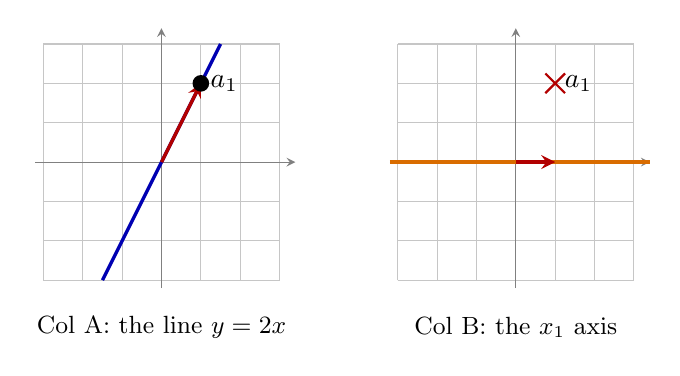
\begin{tikzpicture}[x=0.5cm,y=0.5cm,>=stealth]
  \draw[gray!45] (-3,-3) grid[step=1] (3,3);
  \draw[->,gray] (-3.2,0)--(3.4,0);
  \draw[->,gray] (0,-3.2)--(0,3.4);
  \draw[very thick,blue!70!black] (-1.5,-3)--(1.5,3);
  \draw[->,very thick,red!70!black] (0,0)--(1,2);
  \fill (1,2) circle (3pt);
  \node[right] at (1,2) {$a_1$};
  \node at (0,-4.2) {\small Col A: the line $y=2x$};
  \begin{scope}[shift={(9,0)}]
    \draw[gray!45] (-3,-3) grid[step=1] (3,3);
    \draw[->,gray] (-3.2,0)--(3.4,0);
    \draw[->,gray] (0,-3.2)--(0,3.4);
    \draw[very thick,orange!85!black] (-3.2,0)--(3.4,0);
    \draw[->,very thick,red!70!black] (0,0)--(1,0);
    \draw[thick,red!70!black] (0.75,1.75)--(1.25,2.25) (0.75,2.25)--(1.25,1.75);
    \node[right] at (1,2) {$a_1$};
    \node at (0,-4.2) {\small Col B: the $x_1$ axis};
  \end{scope}
\end{tikzpicture}
\end{center}

\textbf{Figure 3.} The column spaces of $A=\begin{bmatrix}1&2\\2&4\end{bmatrix}$ (left) and of $B=\begin{bmatrix}1&2\\0&0\end{bmatrix}$ (right), where $B$ comes from $A$ by $R_2-2R_1$. The vector $\bv{a}_1=(1,2)$ is in the first line; on the right it is not on the $x_1$-axis (a cross marks it). The row operation moved the column space.

\begin{think}{Why row operations keep $\Nul A$ but move $\Col A$}{rowops}
(a)~Why do $A\bv{x}=\bv{0}$ and $B\bv{x}=\bv{0}$ have exactly the same solutions when $B$ is obtained from $A$ by a row operation? Think of what a row operation does to the \emph{equations}. (b)~Now look at what a row operation does to the \emph{columns}. In the proof that $\Row B=\Row A$ the new rows were combinations of the old rows. What is the analogous statement for columns, and why does it fail?
\end{think}

\begin{warn}[Nul A lives in $\R^n$ and Col A lives in $\R^m$]
The two subspaces of a matrix usually live in different spaces. For a $4\times7$ matrix $\Nul A\subseteq\R^7$ and $\Col A\subseteq\R^4$. Writing $\Nul A=\Col A$ or asking whether a vector of $\R^4$ is in $\Nul A$ is a type error: there is nothing to compute. The number of \emph{columns} decides where $\Nul A$ lives; the number of \emph{rows} decides where $\Col A$ lives.
\end{warn}

\begin{warn}[A null space is never empty]
Every null space contains $\bv{0}$, because $A\bv{0}=\bv{0}$. A subspace is never empty, and $\Nul A=\{\bv{0}\}$ is a perfectly good null space with exactly one vector. ``No nonzero solutions'' does not mean ``no solutions''. Likewise the equation $A\bv{x}=\bv{0}$ is always consistent, whereas $A\bv{x}=\bv{b}$ need not be.
\end{warn}

\begin{kc}{Null space or column space?}{nulorcol}
Let $A=\begin{bmatrix}1&2\\2&4\\3&6\end{bmatrix}$. For each vector, say whether it lies in $\Nul A$, in $\Col A$, in both or in neither: (a)~$(-2,1)$; (b)~$(1,2,3)$; (c)~$(2,4,5)$; (d)~$(1,2)$; (e)~$(0,0)$.
\end{kc}

\begin{exmp}{In which $\R^k$ do they live? Null or column space?}{layk}
Let $A=\begin{bmatrix}1&0&2\\0&1&-1\\3&2&4\\2&-1&5\end{bmatrix}$. (a)~Find $k$ such that $\Nul A$ is a subspace of $\R^k$, and $k$ such that $\Col A$ is a subspace of $\R^k$. (b)~Decide whether $\bv{w}=(-2,1,1)$ is in $\Nul A$, and whether $\bv{p}=(1,1,5,1)$ and $\bv{q}=(1,1,5,0)$ are in $\Col A$.

\textbf{Solution.} (a)~$A$ has $3$ columns, so $\Nul A\subseteq\R^3$ and $k=3$. $A$ has $4$ rows, so $\Col A\subseteq\R^4$ and $k=4$.

(b)~Only the multiplication test applies to $\bv{w}$:
\[
A\bv{w}=\begin{bmatrix}1&0&2\\0&1&-1\\3&2&4\\2&-1&5\end{bmatrix}\begin{bmatrix}-2\\1\\1\end{bmatrix}=\begin{bmatrix}-2+0+2\\0+1-1\\-6+2+4\\-4-1+5\end{bmatrix}=\begin{bmatrix}0\\0\\0\\0\end{bmatrix},
\]
so $\bv{w}\in\Nul A$. The vectors $\bv{p}$ and $\bv{q}$ have $4$ entries, so only $\Col A$ can contain them. For $\bv{q}$, row reduce $[A\ \bv{q}]$:
\begin{align*}
\begin{amat}{ccc|c}1&0&2&1\\0&1&-1&1\\3&2&4&5\\2&-1&5&0\end{amat}
&\rops{R_3-3R_1,\ R_4-2R_1}
\begin{amat}{ccc|c}1&0&2&1\\0&1&-1&1\\0&2&-2&2\\0&-1&1&-2\end{amat}\\[4pt]
&\rops{R_3-2R_2,\ R_4+R_2}
\begin{amat}{ccc|c}1&0&2&1\\0&1&-1&1\\0&0&0&0\\0&0&0&-1\end{amat}.
\end{align*}
The last row says $0=-1$, so $\bv{q}\notin\Col A$. For $\bv{p}$ no reduction is needed if we spot a solution: $A(1,1,0)=(1+0,\ 0+1,\ 3+2,\ 2-1)=(1,1,5,1)=\bv{p}$, the sum of the first two columns, so $\bv{p}\in\Col A$.
\end{exmp}

\begin{exmp}{Is this set a subspace? Write it as a null space or a column space}{laysub}
\textbf{(a)} Let $W=\{(a,b,c,d):\ a-2b+5c=d\text{ and }c-a=b\}$. Moving everything to the left, $W$ is the set of solutions of
\[
a-2b+5c-d=0,\qquad -a-b+c=0,\qquad\text{that is,}\qquad \begin{bmatrix}1&-2&5&-1\\-1&-1&1&0\end{bmatrix}\begin{bmatrix}a\\b\\c\\d\end{bmatrix}=\begin{bmatrix}0\\0\end{bmatrix}.
\]
So $W=\Nul A$ for a $2\times4$ matrix $A$, and $W$ is a subspace of $\R^4$ by Theorem~\ref{thm:nulsub}, with no further work.

\textbf{(b)} Let $V=\{(r+2s,\ 2r-t,\ s+t,\ 3r):\ r,s,t\in\R\}$. Splitting by parameters,
\[
(r+2s,\ 2r-t,\ s+t,\ 3r)=r\begin{bmatrix}1\\2\\0\\3\end{bmatrix}+s\begin{bmatrix}2\\0\\1\\0\end{bmatrix}+t\begin{bmatrix}0\\-1\\1\\0\end{bmatrix},
\]
so $V=\Col A$ for the $4\times3$ matrix $A$ with these three columns, and $V$ is a subspace of $\R^4$ by Theorem~\ref{thm:colsub}.

\textbf{(c)} Let $S=\{\bv{x}\in\R^3:\ x_1+x_2+x_3=1\}$. This is the solution set of $A\bv{x}=\bv{b}$ with $A=\begin{bmatrix}1&1&1\end{bmatrix}$ and $\bv{b}=(1)$, with $\bv{b}\neq\bv{0}$. It is \emph{not} a null space, and it is not a subspace: $A\bv{0}=\bv{0}\neq\bv{b}$, so $\bv{0}\notin S$.

\textbf{(d)} Let $T=\{(a,b):\ ab=0\}$. No matrix helps here: the condition $ab=0$ is not a system of linear equations in $a,b$, and $T$ is the union of the axes (Example~\ref{4.1-ex:shapes}), which is not a subspace. A set can be recognised as a subspace by writing it as a null space or a column space, but a set that cannot be written either way has to be tested directly.
\end{exmp}

% ---------------------------------------------------------------------
\subsection*{Linear transformations of vector spaces}

In Section 1.8 a linear transformation was a map $T:\R^n\to\R^m$ that preserves sums and scalar multiples. Nothing in those two rules uses entries, so they make sense for any pair of vector spaces. (The remark at the end of Section 1.8 anticipated exactly this.)

\begin{defn}{Linear transformation}{lintrans}
Let $V$ and $W$ be vector spaces. A \emph{linear transformation} $T:V\to W$ is a rule that assigns to each vector $\bv{v}$ in $V$ a unique vector $T(\bv{v})$ in $W$ such that, for all $\bv{u},\bv{v}$ in $V$ and all scalars $c$,
\begin{enumerate}[label=(\roman*),itemsep=1pt]
  \item $T(\bv{u}+\bv{v})=T(\bv{u})+T(\bv{v})$, and
  \item $T(c\bv{u})=c\,T(\bv{u})$.
\end{enumerate}
The space $V$ is the \emph{domain} and $W$ the \emph{codomain} of $T$ (Definition~\ref{1.8-def:transf}). For $V=\R^n$ and $W=\R^m$ this is Definition~\ref{1.8-def:linear}.
\end{defn}

In (i) the sum on the left is a sum in $V$ and the sum on the right is a sum in $W$; in (ii) likewise for the scalar multiples. Different spaces, different operations, same symbols.

\begin{thm}{First consequences of linearity}{ltbasic}
Let $T:V\to W$ be a linear transformation. Then
\begin{enumerate}[label=(\alph*),itemsep=1pt]
  \item $T(\bv{0})=\bv{0}$ (the zero vector of $V$ goes to the zero vector of $W$);
  \item $T(c\bv{u}+d\bv{v})=c\,T(\bv{u})+d\,T(\bv{v})$ for all $\bv{u},\bv{v}$ in $V$ and scalars $c,d$;
  \item $T(-\bv{u})=-T(\bv{u})$ and $T(\bv{u}-\bv{v})=T(\bv{u})-T(\bv{v})$.
\end{enumerate}
\end{thm}

\begin{proof}
(a)~By Theorem~\ref{4.1-thm:conseq}(c) in $V$, $\bv{0}=0\cdot\bv{0}$. Then by (ii), $T(\bv{0})=T(0\cdot\bv{0})=0\cdot T(\bv{0})$, and $0\cdot T(\bv{0})$ is the zero vector of $W$ by Theorem~\ref{4.1-thm:conseq}(c) in $W$. (b)~$T(c\bv{u}+d\bv{v})=T(c\bv{u})+T(d\bv{v})=cT(\bv{u})+dT(\bv{v})$ by (i) and (ii). (c)~By Theorem~\ref{4.1-thm:conseq}(e), $-\bv{u}=(-1)\bv{u}$, so $T(-\bv{u})=T((-1)\bv{u})=(-1)T(\bv{u})=-T(\bv{u})$; then $T(\bv{u}-\bv{v})=T(\bv{u}+(-1)\bv{v})=T(\bv{u})-T(\bv{v})$ by (b).
\end{proof}

Part (a) is Theorem~\ref{1.8-thm:props}(a) again, now proved from the vector space axioms only. It gives a fast test for non-examples: if $T(\bv{0})\neq\bv{0}$, then $T$ is not linear.

\begin{exmp}{A matrix map, seen as a linear transformation of vector spaces}{matmap}
Let $A$ be an $m\times n$ matrix and $T(\bv{x})=A\bv{x}$ from $\R^n$ to $\R^m$. This is a linear transformation (Theorem~\ref{1.8-thm:matlin}). Take $A$ to be the matrix of Example~\ref{ex:contrast}, so $T:\R^4\to\R^3$. The vectors sent to $\bv{0}$ are the solutions of $A\bv{x}=\bv{0}$, the set $\Nul A$, which we found to be $\Span\{(-1,-1,1,0),(-2,3,0,1)\}$. The set of all outputs $T(\bv{x})=A\bv{x}$ is $\Col A$ (Theorem~\ref{thm:colsub}(b)), the plane $3b_1-b_2+b_3=0$. So for a matrix map the two sets that we are about to define for a general $T$ are exactly the null space and the column space.
\end{exmp}

\begin{defn}{Kernel and range}{kerrange}
Let $T:V\to W$ be a linear transformation. The \emph{kernel} of $T$ is the set of all vectors of $V$ that $T$ sends to the zero vector of $W$:
\[
\ker T=\{\bv{v}\in V:\ T(\bv{v})=\bv{0}\}.
\]
The \emph{range} of $T$ is the set of all images:
\[
\operatorname{range}T=\{T(\bv{v}):\ \bv{v}\in V\}.
\]
\end{defn}

The kernel is a subset of the domain $V$ and the range is a subset of the codomain $W$. For $T(\bv{x})=A\bv{x}$ they are $\Nul A\subseteq\R^n$ and $\Col A\subseteq\R^m$.

\begin{thm}{Kernel and range are subspaces}{kersub}
Let $T:V\to W$ be a linear transformation. Then $\ker T$ is a subspace of $V$ and $\operatorname{range}T$ is a subspace of $W$.
\end{thm}

\begin{proof}
\emph{Kernel.} By Theorem~\ref{thm:ltbasic}(a), $T(\bv{0})=\bv{0}$, so $\bv{0}$ is in $\ker T$. If $\bv{u},\bv{v}$ are in $\ker T$, then $T(\bv{u}+\bv{v})=T(\bv{u})+T(\bv{v})=\bv{0}+\bv{0}=\bv{0}$ and $T(c\bv{u})=cT(\bv{u})=c\bv{0}=\bv{0}$, so $\bv{u}+\bv{v}$ and $c\bv{u}$ are in $\ker T$.

\emph{Range.} The zero vector of $W$ is $T(\bv{0})$, so it is in the range. If $\bv{w}_1=T(\bv{u}_1)$ and $\bv{w}_2=T(\bv{u}_2)$ are in the range, then $\bv{w}_1+\bv{w}_2=T(\bv{u}_1+\bv{u}_2)$ and $c\bv{w}_1=T(c\bv{u}_1)$ are images of vectors of $V$, hence in the range.
\end{proof}

For $T(\bv{x})=A\bv{x}$ the theorem proves once more that $\Nul A$ and $\Col A$ are subspaces. The point of the general proof is that it uses only (i), (ii) and the vector space axioms, so it applies to every linear transformation, including those below, where no matrix is in sight.

\begin{thm}{One-to-one if and only if the kernel is zero}{onetoone}
A linear transformation $T:V\to W$ is \emph{one-to-one} (that is, $T(\bv{u})=T(\bv{v})$ implies $\bv{u}=\bv{v}$) if and only if $\ker T=\{\bv{0}\}$.
\end{thm}

\begin{proof}
Suppose $T$ is one-to-one and $\bv{v}$ is in $\ker T$. Then $T(\bv{v})=\bv{0}=T(\bv{0})$ by Theorem~\ref{thm:ltbasic}(a), so $\bv{v}=\bv{0}$. Hence $\ker T=\{\bv{0}\}$. Conversely suppose $\ker T=\{\bv{0}\}$ and $T(\bv{u})=T(\bv{v})$. By Theorem~\ref{thm:ltbasic}(c), $T(\bv{u}-\bv{v})=T(\bv{u})-T(\bv{v})=\bv{0}$, so $\bv{u}-\bv{v}$ is in $\ker T$, hence $\bv{u}-\bv{v}=\bv{0}$ and $\bv{u}=\bv{v}$.
\end{proof}

This generalises Theorem~\ref{1.9-thm:ontoone}(a), where $T(\bv{x})=\bv{0}$ having only the trivial solution was equivalent to one-to-one, and Theorem~\ref{1.8-thm:sameimage}, where $T(\bv{x})=T(\bv{y})$ was equivalent to $T(\bv{x}-\bv{y})=\bv{0}$. Likewise $T$ is \emph{onto} $W$ (Definition~\ref{1.9-def:ontoone}) exactly when $\operatorname{range}T=W$.

\begin{think}{Why the kernel decides injectivity}{onetoone}
In your own words, explain why ``$T$ is one-to-one if and only if $\ker T=\{\bv{0}\}$'' is true. Where in the proof is linearity used? Is the statement true for a function $f:\R\to\R$ that is not linear, say $f(x)=x^2$ with $f(x)=0$ only for $x=0$?
\end{think}

\begin{think}{Can a kernel be empty?}{empty}
A student writes, ``The kernel of this map is empty, so the map is one-to-one.'' What is wrong with the sentence? What is the correct statement, and which result guarantees that the kernel of a linear transformation is never empty?
\end{think}

\begin{exmp}{Differentiation on polynomials}{ltD}
Let $D:\mathbb{P}_3\to\mathbb{P}_2$ be $D(p)=p'$ (the derivative; Example~\ref{1.8-ex:poly} treated differentiation on polynomials through coefficient vectors). The rules $(p+q)'=p'+q'$ and $(cp)'=c\,p'$ are (i) and (ii), so $D$ is linear.

\emph{Kernel.} For $p=a_0+a_1t+a_2t^2+a_3t^3$ we have $D(p)=a_1+2a_2t+3a_3t^2$, which is the zero polynomial if and only if $a_1=a_2=a_3=0$. So $\ker D=\{a_0\}=\Span\{1\}$, the constant polynomials. \emph{Range.} Given $q=b_0+b_1t+b_2t^2$ in $\mathbb{P}_2$, the polynomial $p=b_0t+\tfrac12b_1t^2+\tfrac13b_2t^3$ in $\mathbb{P}_3$ has $D(p)=q$. So $\operatorname{range}D=\mathbb{P}_2$ and $D$ is onto.

Since $\ker D\neq\{\bv{0}\}$, Theorem~\ref{thm:onetoone} says $D$ is not one-to-one, and indeed $D(1)=D(2)=\bv{0}$, or $D(t^2)=D(t^2+7)=2t$: two polynomials with the same derivative differ by a constant.
\end{exmp}

\begin{exmp}{Evaluation of a polynomial at a point}{ltEval}
Let $E:\mathbb{P}_2\to\R$ be $E(p)=p(1)$. Then $(p+q)(1)=p(1)+q(1)$ and $(cp)(1)=c\,p(1)$, so $E$ is linear. Here the codomain is $\R$, the vector space of all real numbers.

\emph{Kernel.} $p=a_0+a_1t+a_2t^2$ is in $\ker E$ if and only if $a_0+a_1+a_2=0$, that is, $a_0=-a_1-a_2$, and then $p=a_1(t-1)+a_2(t^2-1)$. So $\ker E=\Span\{t-1,\ t^2-1\}$. (The map $p\mapsto p(0)$ has kernel $\Span\{t,t^2\}$; compare Example~\ref{4.1-ex:polysub}(a).) \emph{Range.} The constant polynomial $c$ has $E(c)=c$, so $\operatorname{range}E=\R$ and $E$ is onto. It is not one-to-one, because its kernel is not zero: $E(t-1)=0=E(0)$ with $t-1\neq\bv{0}$.
\end{exmp}

\begin{exmp}{Transpose and trace on $M_{2\times2}$}{ltMat}
\textbf{(a) Transpose.} Let $\tau:M_{2\times2}\to M_{2\times2}$ be $\tau(A)=A\T$. By Theorem~\ref{2.1-thm:transprops}, $(A+B)\T=A\T+B\T$ and $(cA)\T=cA\T$, so $\tau$ is linear. \emph{Kernel:} $A\T=\mathbf{0}$ forces $A=\mathbf{0}$, so $\ker\tau=\{\mathbf{0}\}$ and $\tau$ is one-to-one by Theorem~\ref{thm:onetoone}. \emph{Range:} every matrix $B$ equals $\tau(B\T)$, because $(B\T)\T=B$, so $\operatorname{range}\tau=M_{2\times2}$ and $\tau$ is onto.

\textbf{(b) Trace.} Let $\operatorname{tr}:M_{2\times2}\to\R$ be $\operatorname{tr}\begin{bmatrix}a&b\\c&d\end{bmatrix}=a+d$. Then $\operatorname{tr}(A+B)=\operatorname{tr}A+\operatorname{tr}B$ and $\operatorname{tr}(cA)=c\operatorname{tr}A$, so the trace is linear. \emph{Kernel:} the matrices with $a+d=0$, the trace-zero matrices of Example~\ref{4.1-ex:matsub}(b), $\Span\Bigl\{\begin{bmatrix}1&0\\0&-1\end{bmatrix},\begin{bmatrix}0&1\\0&0\end{bmatrix},\begin{bmatrix}0&0\\1&0\end{bmatrix}\Bigr\}$. \emph{Range:} $\operatorname{tr}\begin{bmatrix}c&0\\0&0\end{bmatrix}=c$, so the range is $\R$. The map is onto and not one-to-one.
\end{exmp}

\begin{exmp}{Symmetrising a matrix}{ltSym}
Let $S:M_{2\times2}\to M_{2\times2}$ be $S(A)=A+A\T$. For $A=\begin{bmatrix}a&b\\c&d\end{bmatrix}$,
\[
S(A)=\begin{bmatrix}a&b\\c&d\end{bmatrix}+\begin{bmatrix}a&c\\b&d\end{bmatrix}=\begin{bmatrix}2a&b+c\\b+c&2d\end{bmatrix}.
\]
$S$ is linear: $S(A+B)=(A+B)+(A+B)\T=(A+A\T)+(B+B\T)=S(A)+S(B)$ by Theorem~\ref{2.1-thm:transprops}, and $S(cA)=cS(A)$.

\emph{Kernel.} $S(A)=\mathbf{0}$ means $2a=0$, $b+c=0$, $2d=0$, so $a=d=0$ and $c=-b$:
\[
\ker S=\left\{\begin{bmatrix}0&b\\-b&0\end{bmatrix}\right\}=\Span\left\{\begin{bmatrix}0&1\\-1&0\end{bmatrix}\right\},
\]
the \emph{skew-symmetric} matrices ($A\T=-A$). \emph{Range.} Every $S(A)$ is symmetric, since its $(1,2)$ and $(2,1)$ entries are equal. Conversely, if $\Sigma$ is any symmetric matrix then $\Sigma\T=\Sigma$ and $S(\tfrac12\Sigma)=\tfrac12\Sigma+\tfrac12\Sigma=\Sigma$. So
\[
\operatorname{range}S=\{\text{symmetric matrices}\}=\Span\left\{\begin{bmatrix}1&0\\0&0\end{bmatrix},\begin{bmatrix}0&1\\1&0\end{bmatrix},\begin{bmatrix}0&0\\0&1\end{bmatrix}\right\}
\]
(Example~\ref{4.1-ex:restriction}(c)). The kernel is not zero, so $S$ is not one-to-one; the range is not all of $M_{2\times2}$, so $S$ is not onto. For instance $S\begin{bmatrix}1&2\\0&3\end{bmatrix}=S\begin{bmatrix}1&1\\1&3\end{bmatrix}$: two different matrices with the same image, and they differ by an element of the kernel.
\end{exmp}

\begin{exmp}{A map on a function space, and a differential equation}{ltFun}
Let $\mathcal{F}$ be the space of all functions $\R\to\R$ and define $T:\mathcal{F}\to\R^2$ by $T(f)=(f(0),f(1))$. Then $T(f+g)=(f(0)+g(0),\ f(1)+g(1))=T(f)+T(g)$ and $T(cf)=cT(f)$, so $T$ is linear.

\emph{Kernel.} $\ker T=\{f:\ f(0)=0\text{ and }f(1)=0\}$, a subspace of $\mathcal{F}$ by Theorem~\ref{thm:kersub}. It contains $f(t)=t^2-t$ and $f(t)=\sin\pi t$, and many more. \emph{Range.} Given $(a,b)$ in $\R^2$, the function $f(t)=a+(b-a)t$ has $f(0)=a$ and $f(1)=b$, so $\operatorname{range}T=\R^2$ and $T$ is onto. It is far from one-to-one.

A second map: let $L(y)=y''+4y$, defined on twice-differentiable functions. Sums and constant multiples pass through derivatives, so $L$ is linear. Its kernel is the set of solutions of the differential equation $y''+4y=0$. The functions $\cos2t$ and $\sin2t$ are in it, since $(\cos2t)''+4\cos2t=-4\cos2t+4\cos2t=0$ and similarly for $\sin2t$. By Theorem~\ref{thm:kersub} every combination $c_1\cos2t+c_2\sin2t$ is in the kernel too; this is the spring subspace of Example~\ref{4.1-ex:spanfunc}. A course in differential equations shows that these are \emph{all} the solutions, so $\ker L=\Span\{\cos2t,\ \sin2t\}$. Solving a homogeneous linear differential equation is finding a kernel.
\end{exmp}

\begin{exmp}{Maps that are not linear}{ltNon}
\textbf{(a)} $N:\mathbb{P}_2\to\mathbb{P}_2$, $N(p)=p+t$. Then $N(\bv{0})=t\neq\bv{0}$. By Theorem~\ref{thm:ltbasic}(a), $N$ is not linear. (Both properties fail: $N(p+q)=p+q+t$ but $N(p)+N(q)=p+q+2t$.)

\textbf{(b)} $\det:M_{2\times2}\to\R$. Here $\det(2I)=4$ but $2\det I=2$, so (ii) fails: $\det(cA)=c^2\det A$, not $c\det A$. Property (i) fails too: with $E_{11}=\begin{bmatrix}1&0\\0&0\end{bmatrix}$ and $E_{22}=\begin{bmatrix}0&0\\0&1\end{bmatrix}$ we have $\det(E_{11}+E_{22})=\det I=1$, while $\det E_{11}+\det E_{22}=0+0=0$.

\textbf{(c)} $Q:\R^2\to\R^2$, $Q(x_1,x_2)=(x_1,\ x_1x_2)$. Then $Q(\bv{0})=\bv{0}$, so the zero test does not detect it, but (ii) fails: $Q(2,2)=(2,4)$ while $2Q(1,1)=2(1,1)=(2,2)$. A map that passes the zero test may still fail one of the two rules.
\end{exmp}

\begin{kc}{Kernel and range in one line}{kerrange}
Give the kernel and the range of each linear map. (a)~$T:\mathbb{P}_3\to\mathbb{P}_1$, $T(p)=p''$. (b)~$T:\R^3\to\R^2$, $T(x_1,x_2,x_3)=(x_1,x_2)$. (c)~$T:\mathcal{F}\to\R$, $T(f)=f(2)$.
\end{kc}

\begin{kc}{Linear or not?}{islinear}
Decide whether each map is linear. If it is not, name the property that fails and give numbers. (a)~$T:\mathbb{P}_2\to\R$, $T(p)=p(0)+1$. (b)~$T:M_{2\times2}\to M_{2\times2}$, $T(A)=A^2$. (c)~$T:\mathbb{P}_2\to\R$, $T(p)=p'(0)$. (d)~$T:\R^2\to\R^2$, $T(x_1,x_2)=(x_2,\ x_1)$.
\end{kc}

\subsection*{Summary}
\begin{itemize}
  \item For an $m\times n$ matrix $A$: $\Nul A=\{\bv{x}\in\R^n:\ A\bv{x}=\bv{0}\}$ is a subspace of $\R^n$ (two proofs: linearity of $A\bv{x}$, and the Subspace Test equation by equation); $\Col A=\Span\{\text{columns}\}=\{A\bv{x}\}=\{\bv{b}:\ A\bv{x}=\bv{b}\text{ consistent}\}$ is a subspace of $\R^m$; $\Row A=\Col A\T$ is a subspace of $\R^n$.
  \item $\Nul A$ is described implicitly. Parametric vector form turns it into a span: one vector for each free variable, and $\Nul A=\{\bv{0}\}$ when there is no free variable. To test a vector, multiply by $A$.
  \item To test whether $\bv{b}\in\Col A$, row reduce $[A\ \bv{b}]$. $\Col A=\R^m$ if and only if there is a pivot in every row; for square matrices this is part of the Invertible Matrix Theorem.
  \item Row operations do not change $\Nul A$ or $\Row A$; they \textbf{do} change $\Col A$. Take spanning vectors for $\Col A$ from the original columns, and read $\Row A$ from the nonzero rows of an echelon form.
  \item A linear transformation $T:V\to W$ between vector spaces satisfies $T(\bv{u}+\bv{v})=T(\bv{u})+T(\bv{v})$ and $T(c\bv{u})=cT(\bv{u})$; then $T(\bv{0})=\bv{0}$. Its kernel is a subspace of $V$ and its range is a subspace of $W$; for $T(\bv{x})=A\bv{x}$ they are $\Nul A$ and $\Col A$.
  \item $T$ is one-to-one if and only if $\ker T=\{\bv{0}\}$, and onto if and only if $\operatorname{range}T=W$.
  \item Examples: differentiation (kernel the constants), evaluation at a point, transpose, trace, $A\mapsto A+A\T$ (kernel the skew-symmetric matrices, range the symmetric ones), $f\mapsto(f(0),f(1))$, and $y\mapsto y''+4y$.
\end{itemize}

\subsection*{Questions to think about before the next section}
\begin{enumerate}
  \item In Example~\ref{ex:nul35} the spanning set for $\Nul A$ has three vectors, one for each free variable. Is any of the three a linear combination of the other two (Section 1.5 made a remark about this)? In Example~\ref{ex:colmember} the third column of $A$ is a combination of the first two. If you delete it, does $\Col A$ change?
  \item Let $T:V\to W$ be linear and suppose $\bv{v}_1,\dots,\bv{v}_p$ span $V$. Do $T(\bv{v}_1),\dots,T(\bv{v}_p)$ span $\operatorname{range}T$?
  \item If $A$ is $n\times n$ and $\Nul A=\{\bv{0}\}$, what is $\Col A$? (Use Theorem~\ref{2.3-thm:imt}.)
\end{enumerate}

\subsection*{Answers and discussion}
\begin{description}[leftmargin=0pt,itemsep=5pt]
  \item[Knowledge Check \ref{kc:shapes}.] The null space lives in $\R^n$ ($n$ columns) and the column space in $\R^m$ ($m$ rows). (a)~$3\times5$: $\Nul A\subseteq\R^5$, $\Col A\subseteq\R^3$. (b)~$4\times2$: $\Nul A\subseteq\R^2$, $\Col A\subseteq\R^4$. (c)~$6\times6$: both in $\R^6$. (d)~$1\times7$: $\Nul A\subseteq\R^7$, $\Col A\subseteq\R^1=\R$.
  \item[Knowledge Check \ref{kc:readnul}.] (a)~The matrix is $2\times3$, so $\Nul A\subseteq\R^3$; $x_3$ is free, $x_1=-3x_3$, $x_2=2x_3$: $\Nul A=\Span\{(-3,2,1)\}$. (b)~$\Nul A\subseteq\R^4$; the pivot columns are $1$ and $3$, the free variables are $x_2,x_4$, with $x_1=-2x_2+x_4$ and $x_3=-4x_4$: $\Nul A=\Span\{(-2,1,0,0),(1,0,-4,1)\}$. (c)~$\Nul A\subseteq\R^2$, both columns are pivot columns: $\Nul A=\{\bv{0}\}$.
  \item[Knowledge Check \ref{kc:surj}.] (a)~Pivots in all three rows (columns $1,2,4$): $\Col A=\R^3$. (b)~The third row has no pivot: $\Col A\neq\R^3$. (c)~The second row is zero and has no pivot: $\Col A\neq\R^3$. In (a) the matrix has more columns than rows, which is necessary but not sufficient; (b) and (c) have no pivot in some row.
  \item[Knowledge Check \ref{kc:nulorcol}.] $A$ is $3\times2$, so $\Nul A\subseteq\R^2$ and $\Col A\subseteq\R^3$. (a)~$(-2,1)$: $A(-2,1)=(-2+2,\ -4+4,\ -6+6)=\bv{0}$, so it is in $\Nul A$; it has $2$ entries, so it cannot be in $\Col A$. (b)~$(1,2,3)$ is the first column of $A$: in $\Col A$ (and it cannot be in $\Nul A$, having $3$ entries). (c)~$(2,4,5)$: in $\R^3$, so only $\Col A$ is possible; every vector of $\Col A$ is a multiple of $(1,2,3)$ (the second column is twice the first), and $(2,4,5)$ is not: neither. (d)~$(1,2)$: $A(1,2)=(5,10,15)\neq\bv{0}$, so not in $\Nul A$, and it is not in $\Col A$ because it has $2$ entries: neither. (e)~The zero vector of $\R^2$ is in $\Nul A$; the zero vector of $\R^3$ is in $\Col A$. The two zero vectors are different vectors (Warning above).
  \item[Knowledge Check \ref{kc:kerrange}.] (a)~$\ker T=\{p:\ p''=0\}=\{a_0+a_1t\}=\mathbb{P}_1$. Range: $a_2t^2+a_3t^3$ has second derivative $2a_2+6a_3t$, which gives every polynomial of $\mathbb{P}_1$, so $\operatorname{range}T=\mathbb{P}_1$. (b)~$\ker T=\{(0,0,x_3)\}=\Span\{(0,0,1)\}$, the $x_3$-axis; $\operatorname{range}T=\R^2$. (c)~$\ker T=\{f:\ f(2)=0\}$; $\operatorname{range}T=\R$ (the constant function $c$ has $f(2)=c$).
  \item[Knowledge Check \ref{kc:islinear}.] (a)~Not linear: $T(\bv{0})=0+1=1\neq0$; the zero test fails. (b)~Not linear: with $A=I$, $T(2I)=4I$ but $2T(I)=2I$, so (ii) fails (and $T(I+I)=4I\neq T(I)+T(I)=2I$, so (i) fails). (c)~Linear: $(p+q)'(0)=p'(0)+q'(0)$ and $(cp)'(0)=c\,p'(0)$. (d)~Linear: it is $\bv{x}\mapsto\begin{bmatrix}0&1\\1&0\end{bmatrix}\bv{x}$, a matrix map.
  \item[Pause and think \ref{think:shifted}.] No. The solution set $\{\bv{x}:\ x_1-2x_2+x_3=2\}$ does not contain $\bv{0}$ (property (a) fails: $0\neq2$), and closure fails too: $(2,0,0)$ and $(0,0,2)$ are solutions but their sum $(2,0,2)$ gives $4\neq2$, and $\tfrac12(2,0,0)=(1,0,0)$ gives $1\neq2$. It is the shifted plane $H_2$ of Example~\ref{4.1-ex:shifted}: by Theorem~\ref{1.5-thm:translate} it is a particular solution $\bv{p}=(2,0,0)$ plus the vectors of $\Nul A$, a \emph{translate} of the subspace $\Nul A$ and not a subspace. The reason in terms of $A$: $A(\bv{u}+\bv{v})=A\bv{u}+A\bv{v}=\bv{b}+\bv{b}=2\bv{b}\neq\bv{b}$ for $\bv{b}\neq\bv{0}$, whereas for $\bv{b}=\bv{0}$ the right side is again $\bv{0}$.
  \item[Pause and think \ref{think:colall}.] (a)~$\Col A=\R^3$, whatever the entries are: a pivot in every row means $A\bv{x}=\bv{b}$ is solvable for every $\bv{b}$ (Theorem~\ref{thm:colall}). (b)~No. A $4\times3$ matrix has at most $3$ pivots, but $\R^4$ needs a pivot in each of the $4$ rows. The columns are only three vectors and cannot span $\R^4$. (c)~If $\Col A\neq\R^n$ then (g) and (h) of Theorem~\ref{2.3-thm:imt} fail, so $A$ is not invertible, and every other statement of the theorem fails too: $A\bv{x}=\bv{0}$ has a nontrivial solution, the columns are dependent, $\det A=0$ and so on.
  \item[Pause and think \ref{think:rowcol}.] For $A=\begin{bmatrix}1&2\\2&4\end{bmatrix}$: $\Row A=\Span\{(1,2),(2,4)\}=\Span\{(1,2)\}$ and $\Col A=\Span\{(1,2),(2,4)\}=\Span\{(1,2)\}$: equal (the matrix is symmetric, so its rows and columns are the same lists). For $A=\begin{bmatrix}0&1\\0&0\end{bmatrix}$: $\Row A=\Span\{(0,1)\}$, the $x_2$-axis, and $\Col A=\Span\{(1,0)\}$, the $x_1$-axis: different. So the two subspaces of $\R^n$ need not coincide; the row space is $\Col A\T$, the column space of a \emph{different} matrix, and they are the same only for special matrices.
  \item[Pause and think \ref{think:rowops}.] (a)~A row operation replaces the system by an equivalent one: the new equations are combinations of the old (interchange, multiples, and an equation plus a multiple of another). Any $\bv{x}$ that satisfies all the old equations satisfies the new ones, and since the operation is reversible, the old equations are combinations of the new ones, so any $\bv{x}$ that satisfies the new equations satisfies the old ones. The right-hand side $\bv{0}$ stays $\bv{0}$. So $\Nul A=\Nul B$. (b)~The analogous statement would be that the columns of $B$ are combinations of the columns of $A$ in the same way. This fails: a row operation mixes the \emph{entries within each column}, not the columns with each other. In Example~\ref{ex:colchange} the column $(1,2)$ of $A$ became $(1,0)$, which is not a multiple of any column of $A$. Hence nothing forces $\Col B\subseteq\Col A$, and in the example $\Col B\neq\Col A$. What does survive is a relation \emph{among the columns of a fixed matrix}: if a column of $A$ is a combination of other columns, the same combination holds in $B$ (because the combination is a solution of the homogeneous system, and $\Nul A=\Nul B$). This is why the pivot positions of $B$ tell us which columns of $A$ to take.
  \item[Pause and think \ref{think:onetoone}.] If two inputs $\bv{u}\neq\bv{v}$ had the same output, then their difference $\bv{u}-\bv{v}$ is a nonzero vector that $T$ sends to $\bv{0}$, so the kernel is bigger than $\{\bv{0}\}$. Conversely, a nonzero vector $\bv{k}$ in the kernel gives two different inputs $\bv{k}$ and $\bv{0}$ with the same output $\bv{0}$. Linearity is used in the step $T(\bv{u}-\bv{v})=T(\bv{u})-T(\bv{v})$: it converts a statement about \emph{pairs} of inputs into a statement about the single vector $\bv{u}-\bv{v}$. For $f(x)=x^2$ the statement is false: $f(x)=0$ only for $x=0$, but $f(2)=f(-2)$. Without linearity, a zero-only kernel does not prevent two inputs from colliding.
  \item[Pause and think \ref{think:empty}.] The sentence is wrong because the kernel of a linear transformation is never empty: $T(\bv{0})=\bv{0}$ (Theorem~\ref{thm:ltbasic}(a)), so $\bv{0}$ is always in the kernel. The correct statement is ``the kernel contains only the zero vector, $\ker T=\{\bv{0}\}$, so the map is one-to-one'' (Theorem~\ref{thm:onetoone}). Also, ``the set is empty'' is never a subspace, because a subspace contains $\bv{0}$.
  \item[Before the next section.] (1)~No vector of the spanning set of Example~\ref{ex:nul35} is a combination of the other two: each free variable $x_j$ appears as a $1$ in its own position in exactly one vector and as a $0$ in the others (see the remark in the example), so a combination of the other two has a $0$ in that position. Deleting the third column of $A$ in Example~\ref{ex:colmember} does not change $\Col A$, since $\bv{a}_3=\bv{a}_1+\bv{a}_2$ is a combination of the others and every combination that uses it can be rewritten without it. (2)~Yes. If $\bv{w}$ is in $\operatorname{range}T$, then $\bv{w}=T(\bv{v})$ for some $\bv{v}=c_1\bv{v}_1+\cdots+c_p\bv{v}_p$, so $\bv{w}=c_1T(\bv{v}_1)+\cdots+c_pT(\bv{v}_p)$ by Theorem~\ref{thm:ltbasic}(b) extended to $p$ terms; and every such combination is in the range. (3)~$\Col A=\R^n$. If $\Nul A=\{\bv{0}\}$ then $A\bv{x}=\bv{0}$ has only the trivial solution, which is (d) of Theorem~\ref{2.3-thm:imt}; hence $A$ is invertible and (h) says that the columns span $\R^n$.
\end{description}

\end{document}
